% !TeX encoding=utf8
% !TeX spellcheck = de_CH_frami

\chapter{BPM in der Domäne "`Home Automation"'}

%---------------------------------------------------------------------------------
\section{Die Domäne "`Home Automation"'}
Im Kontext dieser Arbeit bezeichnet "`Home Automation"' den Gesamten Bereich der Heimautomatisierung im Privat- / Endanwenderbereich. Darunter wird die (teil-) automatisierung von Abläufen im Umfeld rund um das Eigenheim und das Privatleben verstanden.

\begin{figure}[H]
  \centering
  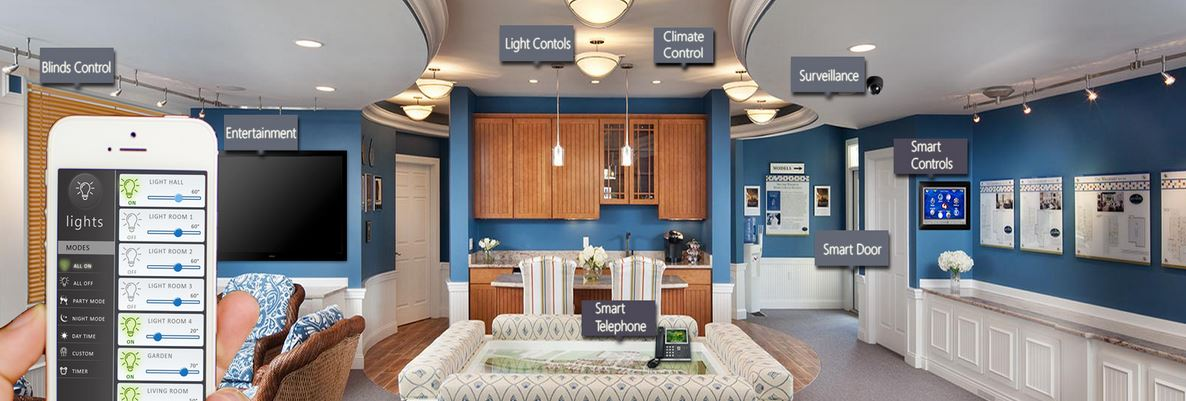
\includegraphics[width=15cm]{./images/home_automation_system}
  \captionsource{Konzeptdarstellung eines "`Smart Home"'}{\url{http://eieihome.com/articles/wp-content/uploads/2015/08/home_automation_system.jpg}}

\end{figure}
"`Home Automation"' oder Heimautomation bezeichnet klassischerweise die Vernetzung und intelligent Kommunikation von Endgeräten in einem "`Eigenheit"'. Das "`Eigenheim"' kann dabei sowohl ein Haus, eine Wohnung oder aber auch ein einzelnes Zimmer oder ähnlich sein. Im weiteren Sinne gehört auch die Automatisierung von grossen Gebäuden, Gebäudekomplexen oder Siedlungen dazu. Dies wird dann aber meistens unter dem Begriff "`Gebäudeautomation"' zusammengefasst.

Bezogen auf die Anwendung im Eigenheim kommt häufig ein bunter Mix an unterschiedlichen Geräten und Technologien zum Einsatz. Dies stellt eine der zentralen Herausforderungen für die autonome Kommunikation der Geräte dar. Durch den Einsatz einer zentralen Koordinationsstelle (z.B. durch einen Home Automation Hub oder ein Smart Gateway) kann hier Abhilfe geschaffen werden. Diese Koordinationsstellen unterstützen in der Regel eine breite Palette an Übertragungs- und Kommunikationsprotokollen und können so zwischen den verschiedenen Endgeräten vermitteln. 

\subsection{Herausforderungen \& Problemstellungen}
Zusätzlich zu den allgemeinen Herausforderungen und Problemstellungen des \gls{acr:IOT} (Sieh dazu das Kapitel \ref{sec:AnalyseIot:ChallangesAndProblems} \nameref{sec:AnalyseIot:ChallangesAndProblems}) hat der Bereich "`Home Automation"' noch eine Reihe spezifischer Herausforderungen und Problemstellungen, welche es zu bewältigen gibt.

\begin{itemize}
\item Einfache Bedienung
\item Integration mit beliebigen Geräten
\item Fehlende Standards und einheitliche Protokolle
\item Vielfalt an Geräten und proprietären Technologien und Protokollen
\item Flexibilität (Exaktes Umfeld der Anwendung ist unbekannt)
\item Zentrale Steuerung
\item Sicherheit
\item Stabilität
\item Zuverlässigkeit
\item Gutes Kosten- / Nutzenverhältnis
\item Geringes technisches Know-How
\end{itemize}

\subsection{Prognose und Zukunft}
Dem Bereich "`Home Automation"' und insbesonder auch "`Smart Home"' wird ein grosses Wachstumspotenzial für die nächsten Jahre prognostiziert. Gartner zufolge könnte im Jahr 2020 eine durchschnittliche Familie über 500 "`Smart Devices"' besitzen \cite{E:Gartner:Prognose:SmartHome}. Beim grössten Teil dieser Geräte wurde es sich um intelligente Haushaltsgeräte handeln. Zu Beginn vorwiegend kleinere Haushaltsgeräte und längerfristig auch zunehmend die grösseren Haushaltsgeräte wie Kühlschränke, Backöfen oder Geschirrspüler. Einer der Schlüssel Aspekte wird gemäss Gartner die Wireless-Technologie sein.

Gemäss Juniper Research werden im Jahr 2020 rund 100 Milliarden US-Dollar für "`Smart Home Services"' (Dienstleistungen und Geräte aus dem Bereich Smart Home) ausgegeben werden. Darin enthalten sind Produkte und Dienstleistungen aus den Bereichen Unterhaltung, Gesundheit, Energie und Heimautomatisierung.

Aufgrund der aktuellen Entwicklung besteht im Bereich "`Smart Home"' und "`Home Automation"' enormes Potenzial für Innovationen und die Erschliessung von neuen Anwendungs- und Geschäftsfeldern. 

%---------------------------------------------------------------------------------
\section{BPM im Kontext von "`Home Automation"'}\ref{sec:Analyse:HA:Kontext}
Der Einsatz von \gls{acr:BPM}, beziehungsweise die dafür verwendeten Notationen \gls{acr:BPMN} und \gls{acr:BPEL}, fokusierte und fokussiert sich nach wie vor primär auf Unternehmen. Aufgrund des notwendigen Know-Hows ist die Verbreitung im Privat-Umfeld nicht sehr hoch. Entsprechend gibt es nur eine eingeschränkte Auswahl an Frameworks, Lösungen und Produkten, welche explizite Funktionalitäten mit \gls{acr:BPMN} oder \gls{acr:BPEL} beinhalten. Viel mehr werden Alternative, beziehungsweise proprietäre Techniken verwendet, um Abläufe zu modellieren. Bei den meisten Lösungen, Produkten oder Frameworks werden Abläufe zu einem grossen Teil in Form von Auslösern (Triggern) und Aktionen (Actions) modelliert. Je nach Produkt können pro Auslöser auch mehrere Aktionen definiert werden, welche sequentiell ablaufen.

Der Vorteil dieser Umsetzung ist die tiefe Einstiegshürde und einfache Verständlichkeit und Erlernbarkeit. Gerade im Umfeld der Heimautomation ist es wichtig, dass sich die Anwendung so einfach als möglich gestaltet. Andernfalls werden die Kunden abgeschreckt und verwenden lieber eine einfacher zu handhabende Lösung.

Der Nachteil und damit der Vorteil von \gls{acr:BPMN} und \gls{acr:BPEL} sind die Plattformneutralität und dadurch die Portabilität. Mit diesen Notationen könnten gängige Abläufe einfach und bequem mit anderen Leuten geteilt werden. Auch wäre die Umstellung auf eine andere Lösung aufgrund der Plattformneutralität relativ bequem möglich. Ebenfalls wird für \gls{acr:BPMN} und \gls{acr:BPEL} spezifisches Fachwissen benötigt, was entsprechend die Einarbeitungszeit erhöht und dadurch die Einstiegsschwelle anhebt.

Das Anwendungsgebiet von Home Automation ist sehr breit gefächert und stark geprägt von den eingesetzten Endgeräten und den genutzten Funktionen. Es gilt in jedem Fall die spezifischen Vor- und Nachteile abzuweägen. Im Nachfolgenden Kapitel werden einige Anwendungsmöglichkeiten aufgezeigt.

Allgemein Betrachtet bietet die Automatisierung und Formalisierung von Abläufen im Home Automation Bereich einige Vorteile. Damit einher gehen aber auch einige Nachteile, welche durch die Nutzung entstehen.



\section{Anwendungsmöglichkeiten}
Für \gls{acr:BPM} oder allgemein die Automatisierung von Abläufen im Bereich des Eigenheimes gibt es eine Reihe von Anwendungsgebieten. Nachfolgend werden einige ausgewählte Szenarien beschrieben:

\begin{itemize}
\itemBfText{Ferienabwesenheit}{Mit einem intelligent vernetzten und automatisierten Eigenheim können viele Tätigkeiten autonom oder via "`Fernbedienung"' durchgeführt werden, für welche andernfalls eine Person zutritt zur Wohnung haben müsste. Nachfolgend werden einige Beispiel aufgelistet.

\begin{itemize}
\item Pflanzengiessen
\item Schliessen der Rollläden am Abend oder bei Sturm
\item Absenkung / Anhebung der Wohnung-Temperatur nach der Abreise / vor der Rückkehr
\item Einbruchsschutz (durch Steuerung von Licht / Ton)
\item Alarmsystem bei einem Notfall
\item Einsparung von Strom (durch automatische Abschaltung nicht benötigter Geräte)
\item Absicherung, dass alle Fenster geschlossen und Herdplatten ausgeschaltet sind
\end{itemize}}

\itemBfText{Schlechtes Wetter / Sturmm}{Im Haushalt befindet sich eine Wetterstation, welche anhand der gesammelten Messwerte und den Vorhersagen und Informationen von lokalen Wetterdienst die aktuelle Wetterlage bestimmen kann. Wird festgestellt, dass ein Sturm aufzieht werden automatisch alle Fenster geschlossen, die Rollläden heruntergelassen und die Sonnenstoren eingefahren. Ist niemand Zuhause werden entsprechende Benachrichtigungen an die Bewohner versandt. Beinhaltet die Vorhersage eine Hagelwarnung oder starke Sturmwarnung könnte der Bewohner zusätzlich informiert werden, dass er zum Beispiel sein Auto in die Garage stellt, um Schäden zu vermeiden.}

\itemBfText{Türklingel}{Klingelt es an der Tür kann das System aufgrund der verbauten Kamera feststellen, wer sich an der Tür befindet. Handelt es sich um eine bekannte Person, welche erwartet wird kann die Türe automatisch geöffnet und der Bewohner entsprechend informiert werden. Handelt es sich um eine unbekannte Person, wird der Bewohner benachrichtigt und die Video- und Sprachverbindung zum Aussenbereich hergestellt. Je nach Entscheid des Bewohners wird der Besucher eingelassen oder nicht. Ist der Bewohner nicht zuhause und jemand klingelt an der Tür, wird der Bewohner via Textnachricht informiert und das Foto des Besuchers für eine spätere Überprüfung gespeichert.}
\end{itemize} 


\section{Lösungen, Produkte, Frameworks, ...}\label{sec:Analyse:HA:LPF}
Im Bereich "`Home Automation"' gibt es aktuell viele verschiedene Lösungen, Produkte und Frameworks. Zum einen handelt es sich um reine Softwarelösungen und zum anderen auch um Kombinationen von Hard- und Software. Wie im Kapitel \ref{sec:Analyse:HA:Kontext} \nameref{sec:Analyse:HA:Kontext} erwähnt, gibt es nur wenige Lösungen, welche eine explizite Prozessunterstützung via \gls{acr:BPMN} oder \gls{acr:BPEL} haben.

\subsection{Software Lösungen}
Nachfolgend werden die Software-Lösungen, Produkte und Frameworks aus dem Bereich "`Home Automation"' aufgelistet, welche durch die Recherche ermittelt wurden. Diese wurden jeweils auf rudimentär auf ausgewählte Eigenschaften hin überprüft. Als Quelle für die Zuordnung der Eigenschaften diente der jeweilige Webauftritt und die dazugehörigen Dokumentationen. Eine detaillierte und tiefer führende Analyse der einzelnen Lösungen wurde nicht durchgeführt (Siehe Kapitel \ref{sec:Abgrenzung} \nameref{sec:Abgrenzung}).

Diese Zuordnung dient in erster Linie dazu, einen groben Überblick über die verschiedenen Lösungen zu schaffen und dadurch eine Basis für den weiteren Verlauf der Arbeit zu erhalten.

\begin{table}[H]
\centering
\begin{tabular}{r | c  | c | c | c | c | c | c | c | c | c | c}
	& \THrot{\textbf{Enduser}}
	& \THrot{\textbf{Technisches Know-How notwendig}}
	& \THrot{\textbf{Cloud-basiert}}
	& \THrot{\textbf{Web-basiert}}
	& \THrot{\textbf{Ready-To-Use}}
	& \THrot{\textbf{Framework}}
	& \THrot{\textbf{Trigger \& Action}}
	& \THrot{\textbf{Workflow / Prozesse}}
	& \THrot{\textbf{BPMN / BPEL}}
	& \THrot{\textbf{Open Source / frei verfügbar}}
	& \THrot{\textbf{Lauffähig unter Raspbian 32-Bit}} \\
\midrule
\hyperlink{https://ifttt.com/}{IFTTT}	
	& 	x
	&	
	&	x		
	& 	x 
	&	x
	&	
	&	x
	&	
	&
	& 	x
	&	\\
\midrule
\hyperlink{https://github.com/foxmask/django-th}{Trigger-Happy (IFTTT Clone)}
	& 	x
	&	(x)
	&			
	& 	x 
	&	x
	&	
	&	x
	&	
	&
	& 	x	
	&	x\\
\midrule
\hyperlink{http://www.theintegratedconnection.com/coco-wireless-home-automation/}{CoCo}
	& 	x
	&	
	&	(x)\footnotemark[1]
	& 	(x)\footnotemark[1]
	&	
	&	
	&	x
	&	
	&
	&	
	&	\footnotemark[2] \\
\midrule
\hyperlink{https://home-assistant.io/}{Home Assistant}
	& 	x
	&	(x)	
	&	
	& 	x
	&	x
	&	
	&	x
	&	
	&
	& 	x
	&	x\\
\midrule
\hyperlink{http://www.control4.com/solutions/smart-home-overview}{Control4}
	&	x
	&	
	&	(x)\footnotemark[1]
	&	\footnotemark[2]
	&
	&
	&	\footnotemark[2]
	&	\footnotemark[2]
	&	\footnotemark[2]
	&	
	&  \footnotemark[2] \\
\midrule
\hyperlink{http://universaal.sintef9013.com/index.php/en/}{universAAL}
	& 
	&	x
	&	
	&	x
	&	
	&	x
	&	x
	&
	&
	&	x 
	&  \footnotemark[2] \\
\midrule
\hyperlink{http://www.indigodomo.com/}{indigo domotics (Pro Version)}	
	& 	x
	& 
	&	
	&	x
	&	x
	&	
	&	x
	&	
	&	
	&
	&	\\
\midrule
\hyperlink{http://www.openhab.org/}{openHAB}
	&	x
	&	x
	&	
	&	x
	&	x
	&	
	&	x
	&	(x)\footnotemark[2])
	&	
	&	x 
	&	x\\
\midrule
\hyperlink{http://www.domogik.org/en/}{Domogik}
	&	x
	&  (x)
	&
	&	x
	&	x
	&
	&	x
	&
	&
	& 	x 
	&   x\\
\midrule
\hyperlink{http://www.opensourceautomation.com/}{Open Source Automation}
	&	x
	&	
	&	
	&	x
	&	x
	&	
	&	\footnotemark[2]
	&	\footnotemark[2]
	&
	&	x 
	& \\
\midrule
\hyperlink{http://www.comfortclick.com/}{Comfortclick bOS}
	&	x
	&	(x)
	&	
	&	\footnotemark[2]
	&	x
	&	
	&	x
	&	x
	&
	&	x 
	&   (x)\footnotemark[3]\\
\midrule
\hyperlink{http://www.castleos.com/}{CastleOS}
	&	x
	&	
	&	
	&	x
	&	x
	&	
	&	x
	&	
	&		
	&	x
	& 	\\
\midrule 
\hyperlink{http://www.homegenie.it/}{HomeGenie}
	& x
	& x
	& 
	& x
	& x
	& 
	& x
	& x
	& 
	& x
	& x\\
	
\midrule
\hyperlink{http://www.freedomotic.com/}{Freedomotic}
	& x
	& 
	& 
	& x\footnotemark[1]
	& x
	& 
	& x
	& x
	& 
	& x
	& x\\
	
\midrule
\hyperlink{https://netbeast.co/}{Netbeast}
	& (x)
	& x
	& 
	& x
	& x
	& x
	& x
	& x
	& 
	& x
	& x \\
	
\midrule
\hyperlink{http://www.domoticz.com/}{Domoticz}
	& x
	& (x)
	& 
	& x
	& x
	& 
	& \footnotemark[2]
	& \footnotemark[2]
	& 
	& x
	& x\\
\bottomrule
\end{tabular}
\end{table}

\footnotetext[1]{Möglich, aber optional}
\footnotetext[2]{Keine Informationen verfügbar}
\footnotetext[3]{Nur mit kostenpflichtiger Hardware.}

\newpage
Die betrachteten Lösungen sind grundsätzlich alle für den Endbenutzer einsetzbar. Es gibt zusätzlich noch Angebote im Bereiche Business-2-Business. Dabei werden Unternehmen ganze Plattformen (Hardware und Software) zur Verfügung gestellt, um eigene Home Automation Lösungen zu konzipieren und zu vertreiben (White Label Produkte).

\subsection{Hardware Lösungen (inkl. abgestimmter Software)}
Kombinierte Lösungen aus Hard- und Software gibt es aktuell auf dem eine ganze Reihe verschiedenster Produkte. Viele davon sind proprietär ausgelegt, sodass diese nur mit Produkten der entsprechenden Produktlinie oder vom selben Hersteller oder dessen Partnern funktionieren. Darüber hinaus gibt es auch Lösungen, welche einen eher generischen Ansatz verfolgen. Dabei können Produkte von unterschiedlichsten Herstellern angeschlossen werden. Voraussetzung ist jeweils, dass das entsprechende Protokoll unterstützt wird.

Nachfolgend werden einige der recherchierten Lösungen aufgelistet. Diese werden jedoch im Rahmen dieser Arbeit nicht weiter betrachtet.

\begin{itemize}
\item Bosch G100 Z-Wave Home Control Gateway
\item Samsung Smart things
\item Qivicon
\item Zoo Automation
\item Throne BMS
\end{itemize}

\subsection{Weitere}
Neben Software basierten und Kombinationen von Hard- und Software Lösungen gibt es auch Bestrebungen Referenz-Architekturen zu schaffen. Eine davon ist zum Beispiel die  \hyperlink{http://www.ubicomp.org/ubicomp2013/adjunct/adjunct/p801.pdf}{Home Blox} Architektur.


